% ****** Start of file apssamp.tex ******
%
%   This file is part of the APS files in the REVTeX 4.2 distribution.
%   Version 4.2a of REVTeX, December 2014
%
%   Copyright (c) 2014 The American Physical Society.
%
%   See the REVTeX 4 README file for restrictions and more information.
%
% TeX'ing this file requires that you have AMS-LaTeX 2.0 installed
% as well as the rest of the prerequisites for REVTeX 4.2
%
% See the REVTeX 4 README file
% It also requires running BibTeX. The commands are as follows:
%
%  1)  latex apssamp.tex
%  2)  bibtex apssamp
%  3)  latex apssamp.tex
%  4)  latex apssamp.tex
%
\documentclass[%
 reprint,
%superscriptaddress,
%groupedaddress,
%unsortedaddress,
%runinaddress,
%frontmatterverbose, 
%preprint,
%preprintnumbers,
%nofootinbib,
%nobibnotes,
%bibnotes,
 amsmath,amssymb,
 aps,
%pra,
%prb,
%rmp,
%prstab,
%prstper,
%floatfix,
]{revtex4-2}

\usepackage{graphicx}% Include figure files
\usepackage{dcolumn}% Align table columns on decimal point
\usepackage{bm}% bold math
\usepackage{physics}
%\usepackage{hyperref}% add hypertext capabilities
%\usepackage[mathlines]{lineno}% Enable numbering of text and display math
%\linenumbers\relax % Commence numbering lines

%\usepackage[showframe,%Uncomment any one of the following lines to test 
%%scale=0.7, marginratio={1:1, 2:3}, ignoreall,% default settings
%%text={7in,10in},centering,
%%margin=1.5in,
%%total={6.5in,8.75in}, top=1.2in, left=0.9in, includefoot,
%%height=10in,a5paper,hmargin={3cm,0.8in},
%]{geometry}

\begin{document}



\title{Project 1}% Force line breaks with \\

\author{Clayton Seitz}

\date{\today}% It is always \today, today,
             %  but any date may be explicitly specified


%\keywords{Suggested keywords}%Use showkeys class option if keyword
                              %display desired
\maketitle

%\tableofcontents

\section{Project 1}

\subsection{}


Here, we are trying to solve for the solutions to Schrodinger's eigenvalue equation:

\begin{equation*}
\hat{H}_{0}\phi_{n} = \epsilon_{n}\phi_{n}
\end{equation*}

By discretizing $\phi_{n}$, each $\phi_{n}$ becomes a finite dimensional vector and we can write $\hat{H}$ explicitly as a matrix. That matrix satisfies

\begin{equation*}
\sum_{j}\bra{i}\hat{H}_{0}\ket{j}\vec{\phi}_{n,j} = \epsilon_{n}\vec{\phi}_{n}
\end{equation*}

wheree $\bra{i}\hat{H}_{0}\ket{j}$ is the matrix element $[H_{0}]_{ij}$. It was shown the Schrodingers wave equation could be expressed in discrete form, as

\begin{equation*}
-t(\phi_{n,i+1} + \phi_{n,i-1}) + (2t+V_{i})\phi_{n,i} = \epsilon_{n}\phi_{n,i}
\end{equation*}

which gives us a relationship between $\phi_{n,i}$ and the neighboring elements $\phi_{n,i-1}$ and $\phi_{n,i+1}$. The eigenvalues equation can then be written as a matrix multiplication

\begin{equation}
\hat{H}_{0}\phi_{n} = \begin{pmatrix}
2t + V_{1} & -t & 0 & \hdots\\
-t & 2t + V_{2} & -t& \hdots\\
0 & -t & 2t + V_{3}& \hdots\\
\vdots & \vdots & \vdots & \ddots
\end{pmatrix}
\begin{pmatrix}
\phi_{n,1}\\
\phi_{n,2}\\
\phi_{n,3}\\
\vdots
\end{pmatrix}
\end{equation}

The full matrix $\hat{H}_{0}$ is shown in Figure 1a. 

\subsection{}

From (1) we can see that the diagonal elements represent the discretized potential $V_{n}$ (plus a constant $2t$ where $t = \frac{\hbar^{2}}{2ma^{2}}$). The off-diagonal elements are just constants with dimension of energy over length squared. The matrix of normalized eigenvectors of $\hat{H}_{0}$ are shown in Figure 1b.

\subsection{}

To show that the eigenvectors form an orthonormal set, We can define a matrix $T$ such that each column of $T$ is one eigenvector $\vec{\phi}_{n}$ of $\hat{H}_{0}$. If the eigenvectors are indeed orthonormal, then

\begin{equation*}
T^{T}T = I
\end{equation*}

This product is shown in Figure 1c, and we can see that the eigenvectors are orthonormal.


\begin{figure}[t!]
\centering
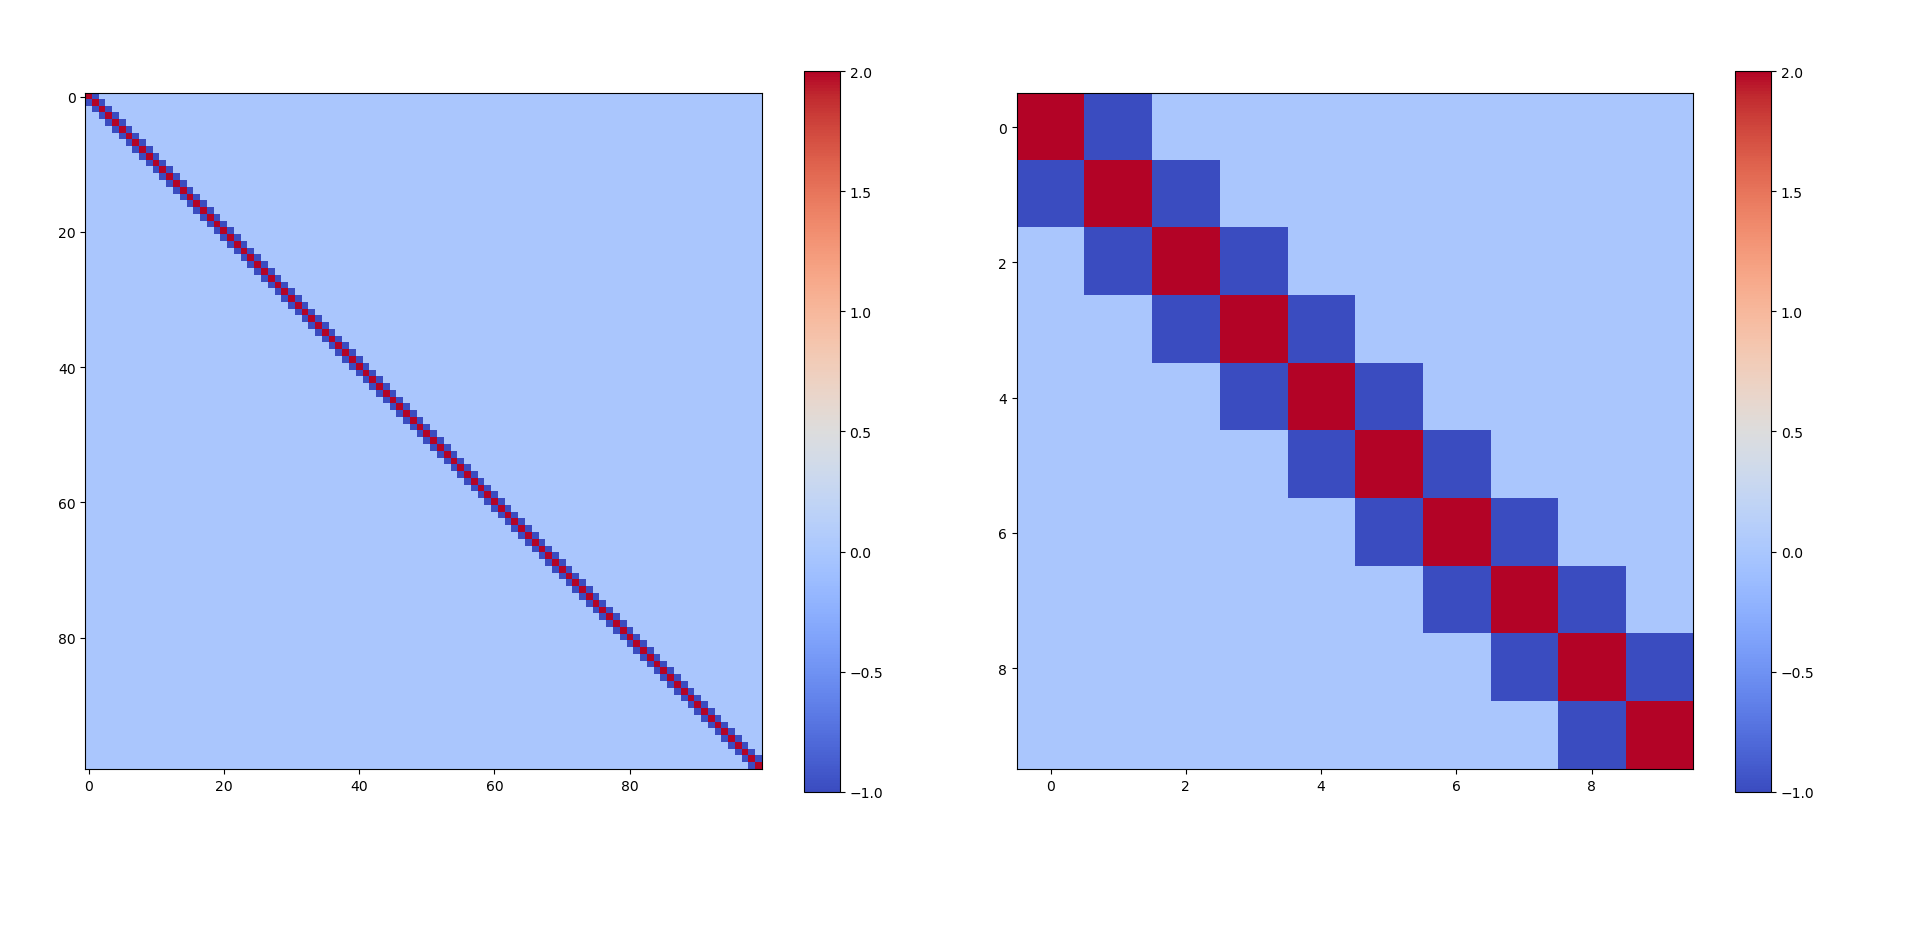
\includegraphics[width=8cm]{p1_1}
\caption{The Hamiltonian matrix for $t=1$}
\label{fig:method}
\end{figure}

\subsection{}

The eigenvalues $\epsilon_{n}$ are shown in Figure 1d in ascending order, indexed by $n$.

\subsection{}

The probability distributions $|\bra{n}\ket{\phi}|^{2}$ for eigenvectors $n = 0, 10, 50$ are shown in the position represention in Figure 2.

\subsection{}

The standard quantum mechanics problem this corresponds to is the free particle in zero potential:

\begin{equation*}
-\frac{\hbar^{2}}{2m}\frac{\partial^{2}\psi}{\partial x^{2}} = E\psi
\end{equation*}

\begin{equation*}
\frac{\partial^{2}\psi}{\partial x^{2}} = -k^{2}\psi
\end{equation*}

for $k = \frac{\sqrt{2mE}}{\hbar}$. So clearly the energy eigenvalues are $E_{k} = \hbar k^{2}/2m$. Notice that $k$ is a continuous parameter and therefore there is a continuum of solutions to the eigenvalue equation. The general solution to the above equation is

\begin{equation*}
\psi(x) = Ae^{ikx}
\end{equation*}

We would expect that the energy eigenvalues in Figure 1d would vary quadratically in $n$; however, the curve has a more sigmoidal shape. Around $n=50$, we can see that the eigenvalues are increasing more linearly because those solutions are actually superpositions of harmonics (See Figure 2, $n=50$ in purple). 

\subsection{}

To understand why, notice that another perfectly valid solution of Schrodinger's equation is


\begin{align*}
\psi(x) &= Ae^{ikx} + Be^{ik'x} \\
&= e^{i(k+k')x/2}\left(Ae^{i(k-k')x/2)} + Be^{-i(k-k')x/2}\right)
\end{align*}

which is a wave with frequency $k-k'$ modulated by the average frequency $(k+k')/2$. 
Furthermore, eigenvalue curve plateaus as $n\rightarrow 100$ because we have chosen a finite sampling frequency $a$, and higher energy solutions cannot be resolved.


\begin{figure}[t!]
\centering
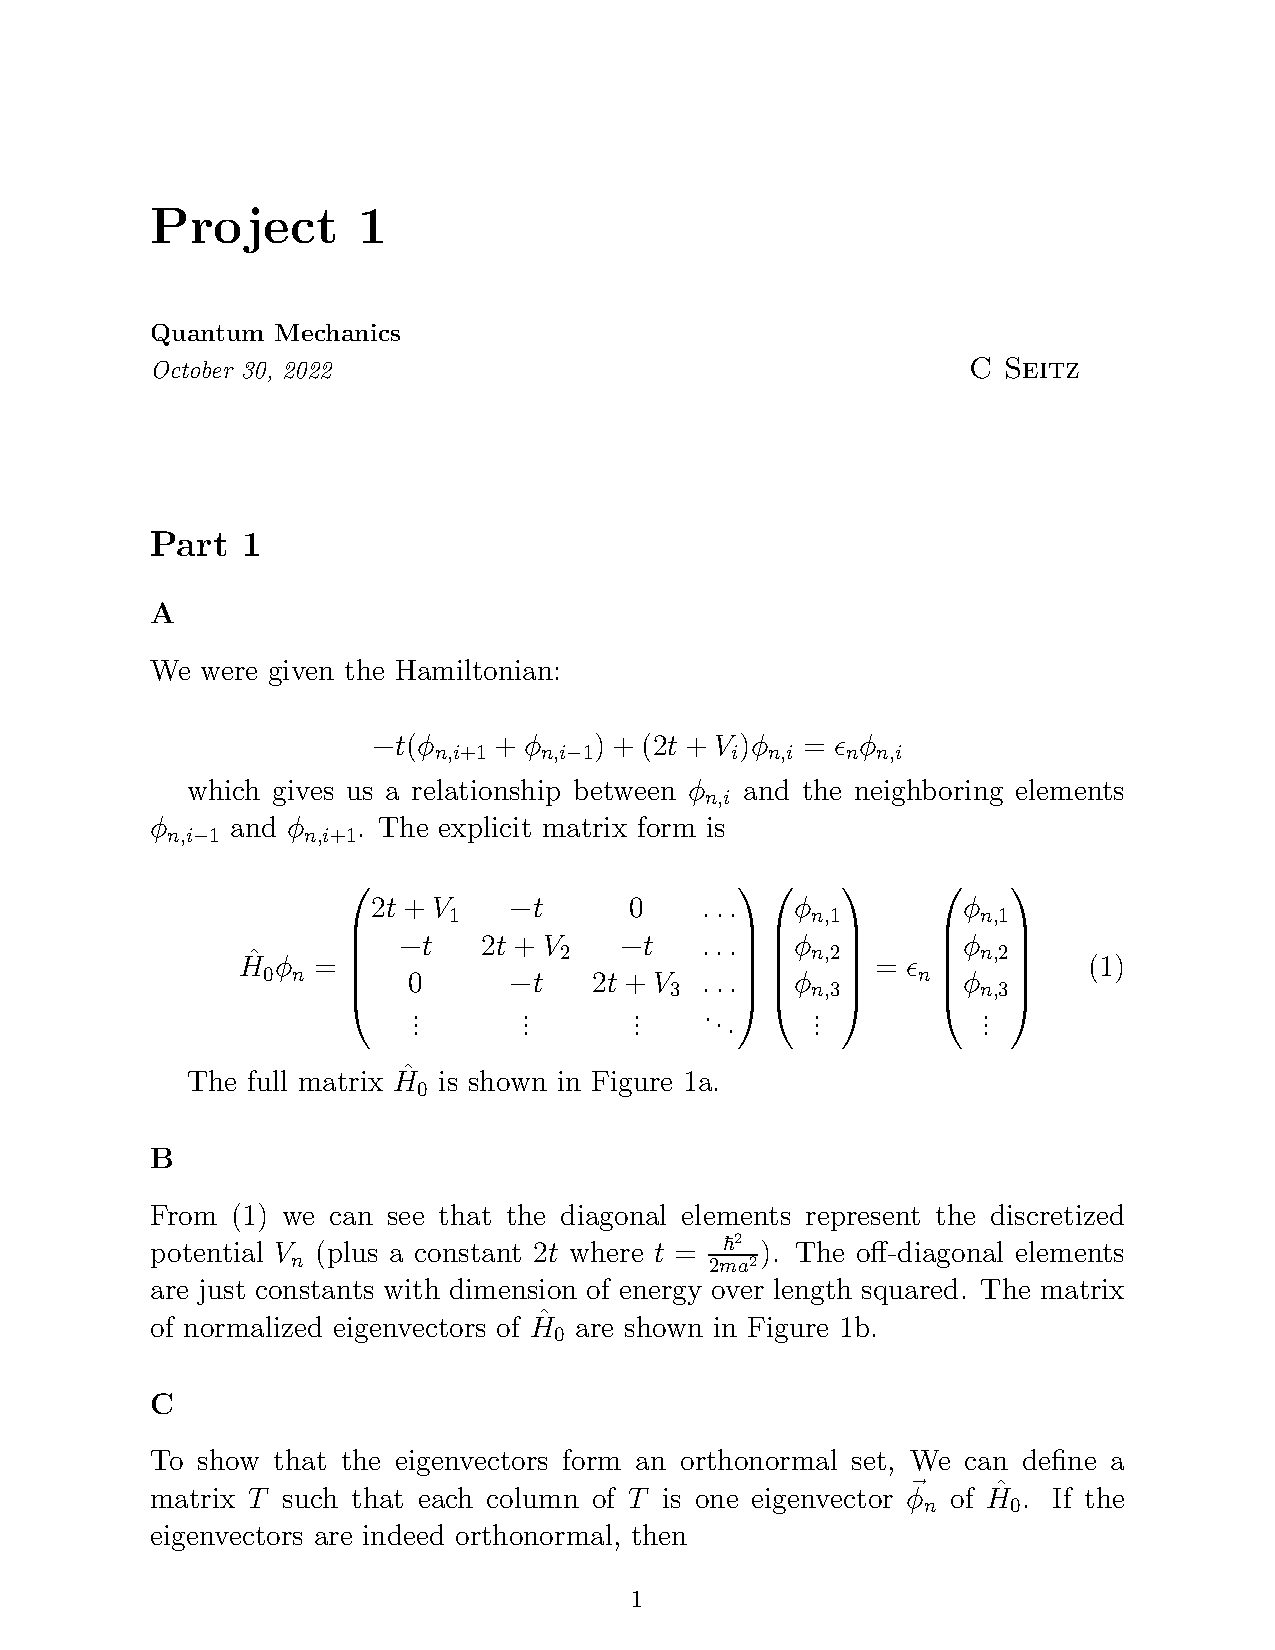
\includegraphics[width=6cm]{p1_2}
\caption{}
\label{fig:method}
\end{figure}

\subsection{}

The unitary operator that transforms $\hat{H_{0}}$ into the $\ket{n}$ basis to the $\ket{\phi_{n}}$ basis is simply

\begin{align*}
U_{0} = T^{-1}
\end{align*}

which we can use to represent our Hamiltonian in the energy basis (we are just diagonalizing the Hamiltonian)

\begin{align*}
\hat{H} = U_{0} H_{0} U_{0}^{-1}
\end{align*}

$\hat{H}$ is shown in Figure 3a, and is diagonal. Of course, this means that the matrix of eigenvectors $T$ is also now a diagonal matrix. The values along the diagonal are $\pm 1$ since the vectors were already shown to be orthonormal and $U_{0}$ was a unitary matrix and therefore preserves orthonormality. The values along the diagonal are $\pm 1$ because there is a phase. Example probability mass functions $|\phi_{n}|^{2}$ are shown in Figure 3d, and are delta functions $\delta(n-n')$, since we have transformed to the energy basis.

\begin{figure}[t!]
\centering
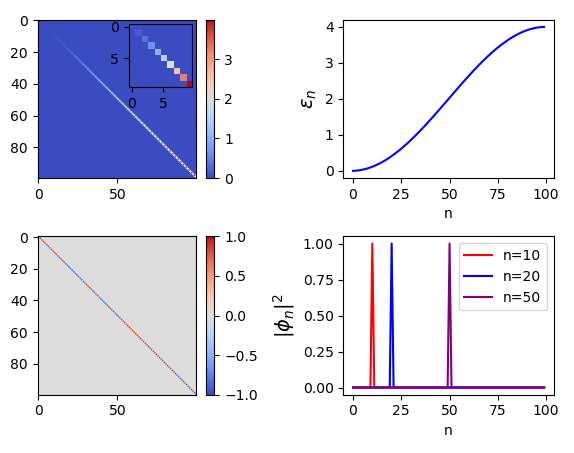
\includegraphics[width=8cm]{p1_3}
\caption{}
\label{fig:method}
\end{figure}

\subsection{}

$\hat{H}$ differs from $\hat{H}_{0}$ from zero to the 29th element and the 69th element to the 100th element along the diagonal. This is because we have set $V=V_{L}$ for $0 \leq x \leq 29a$ and $V=V_{R}$ for $69a\leq x \leq 100$. The matrix $\hat{H}$ is shown in Figure 1a, its sorted eigenvectors are shown in Figure 4b, and their corresponding eigenvalues, sorted in ascending order, are shown in Figure 4d. 

\begin{figure}[t!]
\centering
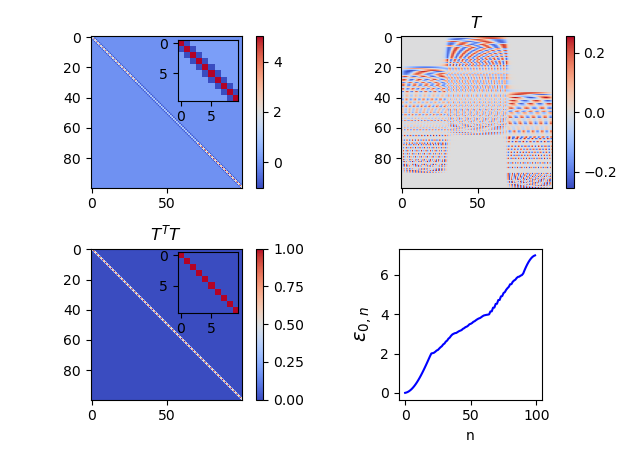
\includegraphics[width=10cm]{p1_5}
\caption{}
\label{fig:method}
\end{figure}

\begin{figure}[t!]
\centering
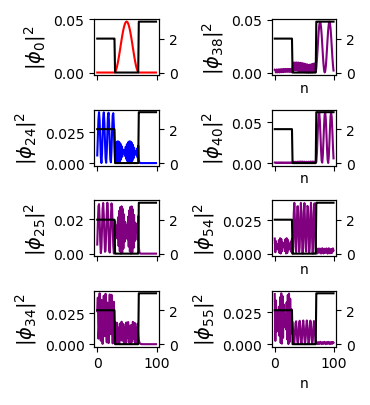
\includegraphics[width=10cm]{p1_6}
\caption{Eigenvectors of the Hamiltonain}
\label{fig:method}
\end{figure}

For $n=0$ a particle is most likely to be in the region where $V=0$, which makes sense because this is the ground state. As we increase the energy for $n=24,25,34$, we see that the particle is no longer bound to the potential well ($E > V_{L}$), but it doesn't have enough energy to be found from $69a\leq x \leq 100$ where $V=V_{R}$ (($E < V_{R}$). So we see decaying exponenitals there. Furthermore, for $n=38,40,54,55$ we see sinusoidal solutions in both regions $0 \leq x \leq 29a$ and $69a\leq x \leq 100$. Clearly the energy is then high enough for the particle to be found there ($E > V_{R}$).

There are kinks in the energy eigenvalue plot because neighboring eigenvectors have more similar energy eigenvalues than before. Presumably this is because the asymmetric shape of the promotes a more discontinuous eigenvalue spectrum.


\begin{figure}[t!]
\centering
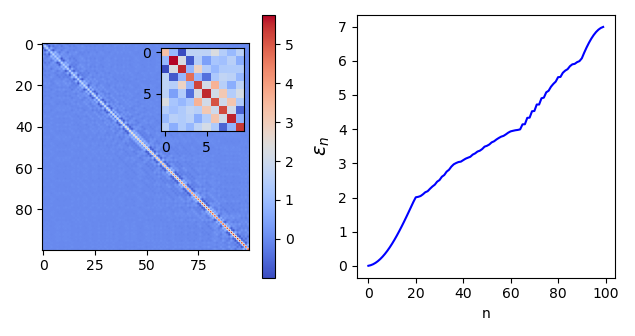
\includegraphics[width=10cm]{p1_7}
\caption{Unitary transformation of $H$ using $U_{0}$}
\label{fig:method}
\end{figure}

The eigenvalue plot for $U_{0}H U_{0}^{-1}$ is the same as for $H$, as they should be. Just because we have changed our representation doesn't change anything physical about the system.

\begin{figure}[t!]
\centering
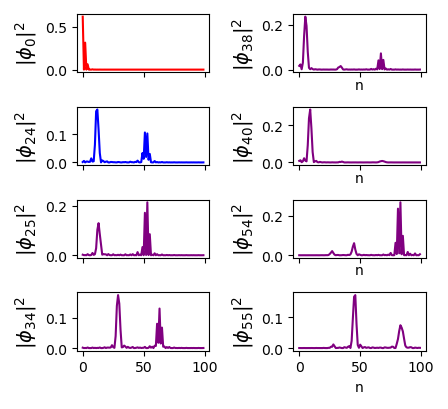
\includegraphics[width=10cm]{p1_8}
\caption{Eigenvectors of $H$ in $H_{0}$ eigenvector basis}
\label{fig:method}
\end{figure}

Physcially the spikes represent components of $\ket{\phi

\end{document}
%
% ****** End of file apssamp.tex ******